\documentclass[aspectratio=169]{beamer}

\title{AMD HIP porting tools and methods}
\author{SURF Open Innovation Lab and University of Amsterdam
				\\In partnership with NIKHEF}
\date{}
\logo{%
    
\includegraphics[width=1cm,height=1cm,keepaspectratio]{img/uvatag}~%
    
\includegraphics[width=2cm,height=2cm,keepaspectratio]{img/sara}%
}%


\usepackage{gnuplottex}
\usepackage{minted}
\usepackage[normalem]{ulem}
\usepackage{graphicx}
\usepackage[binary-units]{siunitx}
\usepackage{hyperref}
\newcommand{\gbs}{\si[per-symbol = \text{~div~}]{\gibi\byte\per\second}}
\newcommand{\hip}{\textbf{\color{red}{hip}}}
\newcommand{\hipblas}{\sout{\color{red}{cu}}\textbf{\color{green}{hip}}}
\newcommand{\HIPBLAS}{\sout{\color{red}{CU}}\textbf{\color{green}{HIP}}}
\begin{document}
\newcommand{\rom}[1]{\uppercase\expandafter{\romannumeral #1\relax}}
\begin{frame}
\titlepage
\end{frame}


% \begin{frame}{Content}
%     \tableofcontents
% \end{frame}{}


\section{Programming models}


\section{HIP}

\begin{frame}{What is HIP}
    \begin{itemize}
        \item Open source C++ runtime API and kernel language
        \item Part of AMD ROCm
        \item Similar programming model to CUDA.
        \item Platform independent (targets NVIDIA and AMD cards)
        \item Feature compariable with CUDA // (in spirit).
    \end{itemize}
\end{frame}

\begin{frame}{What is HIP}
\begin{figure}
    \centering
    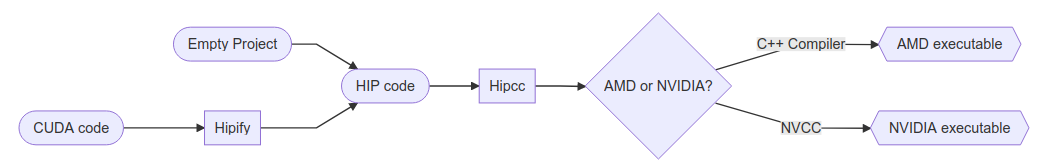
\includegraphics[width=\textwidth]{img/HIP_flow.png}
    % \caption{Caption}
    % \label{fig:my_label}
\end{figure}
\end{frame}

\section{Programming HIP}

\begin{frame}{HIP code example}

\begin{table}[]
    \centering
    \begin{tabular}{l|l|l}
Term & CUDA & HIP\\\hline
Event & cudaEvent\_t & hipEvent\_t\\
Thread-index & threadIdx.x & hipThreadIdx\_x\\
Device kernel & \_\_global\_\_ & \_\_global\_\_\\
Group Memory &  \_\_shared\_\_ & \_\_shared\_\_\\
Constant & \_\_constant\_\_ & \_\_constant\_\_\\
\end{tabular}
    \caption{Term translation table}
    \label{tab:term_translate}
\end{table}

\end{frame}

\begin{frame}[fragile]{HIP code example: vector add}
% \begin{minted}[
% frame=lines,
% framesep=3mm
% ]{c}
% __global__
% void vectorAddKernel(float* deviceA, float* deviceB, float* deviceC){
%     unsigned index = blockIdx.x * blockDim.x + threadIdx.x;
%     deviceC[index] = deviceA[index] + deviceB[index];
% }
% \end{minted}
\begin{minted}[
frame=lines,
framesep=3mm,
escapeinside=||
]{c}
__global__
void vectorAddKernel(float* deviceA, float* deviceB, float* deviceC){
    // unsigned index = blockIdx.x * blockDim.x + threadIdx.x;
    unsigned index = |\hip|BlockIdx_x * |\hip|BlockDim_x + |\hip|ThreadIdx_x;
    deviceC[index] = deviceA[index] + deviceB[index];
}
\end{minted}
\end{frame}

\begin{frame}[fragile]{HIP code example: memory copy}

% \begin{minted}[
% frame=lines,
% framesep=3mm,
% escapeinside=||
% ]{c}
% cudaMalloc((void **) &deviceA, n*sizeof(float));
% cudaMemcpy(deviceA, hostA, n*sizeof(float), cudaMemcpyHostToDevice);
% \end{minted}

\begin{minted}[
frame=lines,
framesep=3mm,
escapeinside=||
]{c}
// cudaMalloc((void **) &deviceA, n*sizeof(float));
// cudaMemcpy(deviceA, hostA, n*sizeof(float), cudaMemcpyHostToDevice);
|\hip|Malloc((void **) &deviceA, n*sizeof(float));
|\hip|Memcpy(deviceA, hostA, n*sizeof(float), |\hip|MemcpyHostToDevice);
\end{minted}
\end{frame}

\begin{frame}[fragile]{HIP code example: kernel launch}

\begin{minted}[
frame=lines,
framesep=3mm,
escapeinside=||
]{c}

// vectorAddKernel<<<n/threadBlockSize, threadBlockSize>>>
//                   (deviceA, deviceB, deviceC);
|{\textbf{\color{red}hipLaunchKernelGGL}}|((vectorAddKernel), 
                   |{\color{red}dim3}|(n/threadBlockSize), |{\color{red}dim3}|(threadBlockSize),
                   0 /*Shared*/, 0/*stream*/,
                   deviceA, deviceB, deviceC);
\end{minted}
\end{frame}

\subsection{Porting code}
\begin{frame}{Hipify}

\begin{itemize}
%    \item Auto-translates a project from CUDA to HIP.
    \item Translates a project from CUDA to HIP.
%    \item It has a Perl version and a Clang version.
    \item Auto-translates most of the calls and kernels.
    \item Reports what it could not change.
    \item Support for most well known CUDA libraries
\end{itemize}
\end{frame}

\begin{frame}{Libraries}
\begin{table}[]
    \centering
    \begin{tabular}{l|l|l}
CUDA & HIP & \\
\hline
cuBLAS &	rocBLAS &	Basic Linear Algebra Subroutines\\
cuFFT &	rocFFT &	Fast Fourier Transfer Library\\
cuSPARSE &	rocSPARSE &	Sparse BLAS + SPMV\\
cuSolver &	rocSolver &	Lapack library\\
AMG-X &	rocALUTION & 	Sparse iterative solvers and preconditioners\\
Thrust& 	hipThrust &	C++ parallel algorithms library\\
CUB &	rocPRIM &	Low Level Optimized Parallel Primitives\\
cuDNN 	&MIOpen &	Deep learning Solver Library\\
cuRAND &	rocRAND &	Random Number Generator Library\\
EIGEN &	EIGEN (Ported) &	C++ template library for linear algebra\\
NCCL &	RCCL &	Communications Primitives Library based on the MPI  \\
\end{tabular}
    \caption{Cuda compatible libraries}
    \label{tab:my_label}
\end{table}
\end{frame}

\begin{frame}{Hipify tools}
\begin{itemize}
    \item \textbf{hipexamine}:
        Scans source directory and reports which files contain CUDA code and how much of the code can automatically be ported.
    \item \textbf{hipify}:
        ``\textit(Hipifies)'' a single file.
    \item \textbf{hipconvertinplace}:
%        Inplace porting of CUDA to HIP of a full directory.
         Ports in-place a full directory from CUDA to HIP.
    \item \textbf{hipify-cmakefile}:
          Translates cmake files to use HIP.
\end{itemize}
\end{frame}


\begin{frame}{Porthing methods}
\begin{itemize}
    \item Hipify-perl 
    \item Hipify-clang
    \item Custom defines to map cuda calls to hip
\end{itemize}
\end{frame}

\begin{frame}{Hipify-perl}
\begin{itemize}
    \item Convert provided files to HIP
    \item Intelligent search replace
    \item Might not work for more complex codes
\end{itemize}

\end{frame}

\begin{frame}{Hipify-clang}
\begin{itemize}
    \item Clang based source parsing
    \item Can replace the compiler to convert a large complex problem
    \item Works better on complex (c++) inputs
\end{itemize}
\end{frame}

\begin{frame}{Using Defines}
\begin{itemize}
    \item Minimal changes needed, only ifdefs for the kernel launches 
    \item No need for a fork of the repo while porting continues.
    \item Easier to integrate in large projects
\end{itemize}
\end{frame}

\begin{frame}[fragile]{HIP code example: Porting Defines}

\begin{minted}[
frame=lines,
framesep=3mm,
escapeinside=||
]{c}
#define cudaMalloc hipMalloc
#define cudaMallocHost hipHostMalloc
#define cudaMemcpy hipMemcpy
#define cudaMemcpyAsync hipMemcpyAsync
#define cudaMemset hipMemset
#define cudaMemsetAsync hipMemsetAsync
#define cudaPeekAtLastError hipPeekAtLastError
#define cudaEventCreate hipEventCreate
#define cudaEventCreateWithFlags hipEventCreateWithFlags
\end{minted}
\end{frame}

\begin{frame}[fragile]{HIP code example: Porting Defines}

\begin{minted}[
frame=lines,
framesep=3mm,
escapeinside=||
]{c}
#if defined(__HIPCC__)
|\color{red}{hipLaunchKernelGGL}|((vectorAddKernel),
                    |\color{red}{dim3}|(n/threadBlockSize), |\color{red}{dim3}|(threadBlockSize),
                    0 /*Shared*/, 0/*stream*/,
                    deviceA, deviceB, deviceC);
#else
vectorAddKernel<<<n/threadBlockSize, threadBlockSize>>>
                 (deviceA, deviceB, deviceC);
#endif
\end{minted}
\end{frame}

\begin{frame}[fragile]{Porting examples}
\begin{itemize}
    \item Porting of Nvidia sample codes
    \item Error checking removed on slides
    \item CuBlAS, FFT and hostcode examples
\end{itemize}
\end{frame}


\begin{frame}[fragile]{Porting examples}
\begin{minted}[
frame=lines,
framesep=3mm,
escapeinside=||
]{c}
|\hipblas|blasCreate(&handle);
|\hipblas|blasSetVector(n2, sizeof(h_A[0]), h_A, 1, d_A, 1);
|\hipblas|blasSetVector(n2, sizeof(h_A[0]), h_A, 1, d_A, 1);
|\hipblas|blasSetVector(n2, sizeof(h_C[0]), h_C, 1, d_C, 1);
|\hipblas|blasSgemm(handle, |\HIPBLAS|BLAS_OP_N, |\HIPBLAS|BLAS_OP_N, N, 
                    N, N, &alpha, d_A,N, d_B, N, &beta, d_C, N);
|\hipblas|blasGetVector(n2, sizeof(h_C[0]), d_C, 1, h_C, 1);
|\hipblas|blasDestroy(handle);
\end{minted}
\end{frame}

\begin{frame}[fragile]{Porting examples}

\begin{minted}[
frame=lines,
framesep=3mm,
escapeinside=||
]{c}
|\hipblas|fftPlan1d(&plan, new_size, |\HIPBLAS|FFT_C2C, 1);
|\hipblas|fftExecC2C(plan, |\hipblas|fftComplex *)d_signal,
                 (|\hipblas|fftComplex *)d_signal, |\HIPBLAS|FFT_FORWARD);
|\hipblas|fftExecC2C(plan, (|\hipblas|fftComplex *)d_filter_kernel,
                 (|\hipblas|fftComplex *)d_filter_kernel, |\HIPBLAS|FFT_FORWARD);
printf("Launching ComplexPointwiseMulAndScale<<< >>>\n");
|\hipblas|LaunchKernelGGL(ComplexPointwiseMulAndScale, dim3(32), dim3(256),
                      0, 0, d_signal, d_filter_kernel,
                      new_size, 1.0f / new_size);
|\hipblas|fftExecC2C(plan, (|\hipblas|fftComplex *)d_signal,
               (|\hipblas|fftComplex *)d_signal, |\HIPBLAS|FFT_BACKWARD);
\end{minted}
\end{frame}

\begin{frame}[fragile]{Hipify-perl output}

\begin{verbatim}
    
info: converted 3 CUDA->HIP refs ( ... )
warn:1 LOC:274 in './simplefft.cpp'
hipMemcpy 3
hipFree 2
HIPFFT_FORWARD 2
hipMemcpyHostToDevice 2
hipMalloc 2
hipDeviceReset 1
hipLaunchKernelGGL 1
HIPFFT_C2C 1
hipMemcpyDeviceToHost 1
HIPFFT_BACKWARD 1
hip_runtime 1
\end{verbatim}
\end{frame}

\begin{frame}[fragile]{Hipify-clang output}

\begin{verbatim}
[HIPIFY] info: file './simplefft.cpp.old' statistics:
CONVERTED refs count: 30
UNCONVERTED refs count: 0
CONVERSION %: 100
REPLACED bytes: 456
TOTAL bytes: 9346
CHANGED lines of code: 20
TOTAL lines of code: 274
CODE CHANGED (in bytes) %: 5
CODE CHANGED (in lines) %: 7
TIME ELAPSED s: 0.17
[HIPIFY] info: CONVERTED refs by type:
[HIPIFY] info: CONVERTED refs by API:
\end{verbatim}
\end{frame}

\begin{frame}{Pitfalls}
\begin{itemize}
    \item \texttt{hipcc} is a lot stricter compared to nvcc
    \item All functions that are called from the device need to be marked as such
    \item Low level optimizations for cuda cards need to be redone
\end{itemize}
\end{frame}

\begin{frame}[fragile]{Conclusion}
\begin{itemize}
    \item HIP enables the development of portable GPU codes
    \item Most CUDA code can be ported to HIP
    \item Tooling is still improving
    \item Performance depends on the kernels
\end{itemize}
\end{frame}


\end{document}

